\section{\bfseries Opis baze podataka}
Baza podataka je projektovana tako da pokrije sve slučajeve upotrebe informacionog sistema aplikacije CarGo. Na slici \ref{fig:bazaPodataka} prikazana je šema baze.

\begin{figure}[H]
\begin{center}
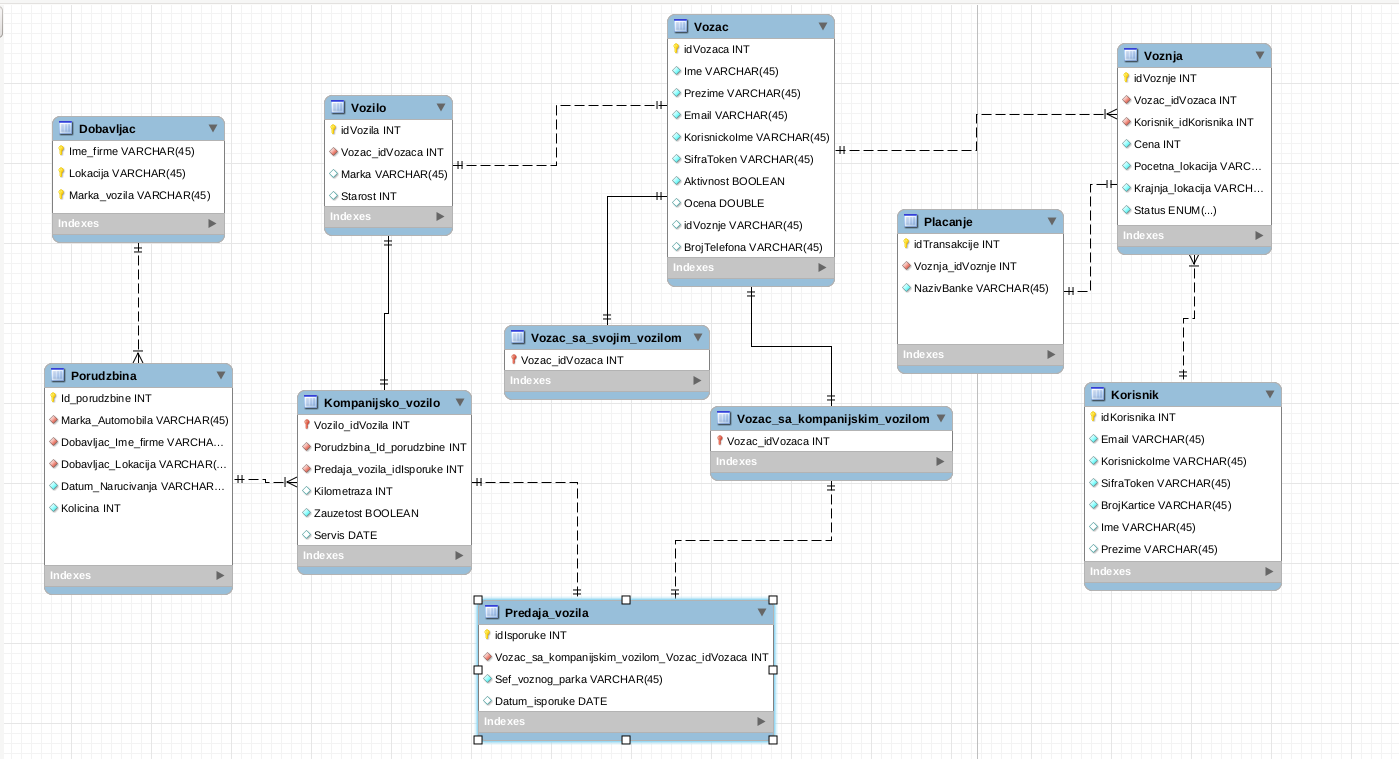
\includegraphics[width=\textwidth]{Slike/EERDijagramBazePodataka.png}
\end{center}
    \caption{Šema baze podataka}
\label{fig:bazaPodataka}
\end{figure}

\subsection{\textbf{Nezavisni entiteti}}
Nezavisni entiteti su:
\begin{itemize}
    \item Vozač
    \item Korisnik
    \item Vozilo
    \item Dobavljač
\end{itemize}

\subsubsection{\textbf{Vozač}}

Svaki vozač ima email i šifru pomoću kojih pristupa svom nalogu. Vozač postaje aktivan kad se prijavi. Atributi:
\begin{itemize}
    \item Ime
    \item Prezime
    \item Ocena - ocena koju je dobio od korisnika u određenoj vožnji
    \item Email - email sa kojim se vozač registrovao
    \item Lozinka - sifra vozača
    \item IdVoznje - vožnje u kojima je vozač učestvovao
\end{itemize}

\subsubsection{\textbf{Korisnik}}

Kao i vozač, i korisnik ima svoj nalog. Korisnik se prijavljuje kad mu je potrebna vožnja. Za registraciju može koristiti ili email ili broj telefona. Iz tog razloga jedna od ove dve kolone može imati vrednost NULL. Atributi:
\begin{itemize}
    \item Ime
    \item Prezime
    \item Email - email korisnika pomoću kojeg se registruje
    \item Mobilni telefon - broj telefona korisnika
    \item Lozinka - šifra korisnika
\end{itemize}

\subsubsection{\textbf{Vozilo}}

Sadrži informacije o vozilima svih vozača. Atributi:
\begin{itemize}
    \item Vozac\_idVozaca - Id vozača koji koristi to vozilo
    \item Marka
    \item Starost
\end{itemize}

\subsubsection{\textbf{Dobavljač}}
Sadrži informacije o dobavljačima od kojih nabavljamo vozila. Atributi:
\begin{itemize}
    \item Ime\_firme
    \item Lokacija
    \item Marka\_vozila
\end{itemize}


\subsection{\textbf{Izvedeni entiteti}}
Izvedeni entiteti su:
\begin{itemize}
    \item Honorarni vozač
    \item Stalno zaposlen vozač
    \item Kompanijsko vozilo
\end{itemize}

\subsubsection{\textbf{Honorarni vozač}}
Predstavlja specijalizaciju eniteta vozač. Sadrži informacije o vozačima koji imaju sopstveno vozilo. Atributi:
\begin{itemize}
    \item Vozac\_idVozaca - Id vozača koji ima sopstveno vozilo, strani ključ ka entitetu vozač
\end{itemize}

\subsubsection{\textbf{Stalno zaposlen vozač}}
Predstavlja specijalizaciju entiteta vozač. Sadrži informacije o vozačima koji nemaju sopstveno vozilo. Atributi:
\begin{itemize}
    \item Vozac\_idVozaca - Id vozača koji nema sopstveno vozilo, strani ključ ka entitetu vozač
\end{itemize}

\subsubsection{\textbf{Kompanijsko vozilo}}
Predstavlja specijalizaciju entiteta vozilo. Sadrži informacije o vozilima koji su u vlasnistvu firme i izdaju se vozačima na korišćenje. Atributi:
\begin{itemize}
    \item Vozilo\_idVozila - strani ključ ka entitetu vozilo.
    \item Porudzbina\_id\_porudzbine - redni broj porudžbine u kojoj je vozilo naručeno
    \item Predaja\_vozila\_idIsporuke - broj isporuke u kojoj je vozilo dostavljeno vozaču.
    \item Kilometraza
    \item Servis
\end{itemize}







